\label{capitolo1}
\section{Progettazione a basso consumo di potenza}
Nel corso degli anni ci si è spostati verso la progettazione di sistemi hardware che consumassero sempre meno. Le motivazioni che hanno portato a questa evoluzione sono molteplici e di diversa natura; alcune di queste sono:
\begin{description}
\item[Tecnologiche:] l'aumento della frequenza e dei transistor presenti nel circuito obbligano ad un minor consumo di energia
\item[Commerciali:] la diffusione di dispositivi portatili che richiedono alte prestazioni e un basso consumo energetico
\item[Economiche:] ridurre il costo del \emph{packaging} del comparto batterie
\end{description}
La diffusione di dispositivi portatili ha portato ad avere un \emph{trade-off} tra le performance ed il consumo energetico.\\
Il design a basso consumo e le metodologie di stima del consumo di potenza devono essere valutate ad un diverso livello di astrazione durante tutto il processo di progettazione; i diversi livelli sono
\begin{itemize}
\item System Level
\item Behavioral Level
\item RT (Register Transfer) Level
\item Gate Level
\item Transistor Level
\end{itemize}
L'evoluzione attuale della tecnologia delle batterie è insufficiente rispetto all'evoluzione odierna dei circuiti, infatti, le capacità delle batterie aumentano all'incirca del 10\%-15\% all'anno mentre il consumo dei circuiti aumenta molto più velocemente, questo comporta un gap notevole tra il fabbisogno di potenza dei circuiti e la disponibilità data dai pacchi batterie.\\
Ad oggi la tecnologia più utilizzata per la realizzazione di circuiti digitali è quella \textbf{CMOS} in quanto la velocità di switching è notevole ed il consumo di corrente è intrinsecamente basso.
Il consumo di potenza nei CMOS è dato da 
$$P=P_{switching}+P_{short-circuit}+P_{leakage}$$
Dove $P_{switching}$ è la potenza necessaria per caricare e scaricare il condensatore durante il cambio di contesto del transistor $P_{short-circuit}$ è la corrente che va da $V_{dd}$ a $GND$ durante la transizione di uscita ed infine $P_{leakage}$ è la componente data dalla corrente di leakage.\\
La parte $P_{switching}$ è la parte predominante della dissipazione di potenza e l'obiettivo dei progettisti è quello di minimizzare questo fattore durante la fase di design del sistema. Per quanto riguarda, invece, $P_{short-circuit}$ e $P_{leakage}$ per minimizzarli occorre agire a livello tecnologico e non risulta essere una cosa semplice.\\
Vediamo ora come caratterizzare in modo più accurato la potenza di switching; distinguiamo inanzi tutto due casi:
\begin{itemize}
\item Transizione da $0 \rightarrow V_{dd}$ Fig. \ref{fig:vddoutput}
\item Transizione da $V_{dd} \rightarrow 0$ Fig. \ref{fig:ooutput}
\end{itemize}
\begin{figure}[hbt]
\begin{minipage}[b]{8cm}
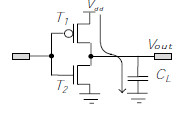
\includegraphics[width=7cm]{img/vddoutput.png}
\caption{Transizione $0 \rightarrow V_{dd}$}\label{fig:vddoutput}
\end{minipage}
\ \hspace{2mm} \hspace{3mm} \
\begin{minipage}[b]{8cm}
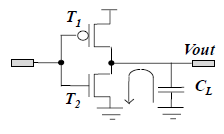
\includegraphics[width=7cm]{img/ooutput.png}
\caption{Transizione $V_{dd} \rightarrow 0$}\label{fig:ooutput}
\end{minipage}
\end{figure}
L'energia dissipata nel primo caso è data da:
\begin{itemize}
\item l'energia dissipata dal PMOS $T_1$ uguale a $\frac{1}{2}C_LV_{dd}^2$
\item l'energia immagazzinata in $C_L$ uguale a $\frac{1}{2}C_LV_{dd}^2$
\item l'energia derivante dalla carica uguale a $C_LV_{dd}^2$
\end{itemize}
Nel secondo caso abbiamo invece un'unica componente di dissipazione che è l'energia dissipata da $T_2$ uguale a $\frac{1}{2}C_LV_{dd}^2$.\\
Se le transizioni $0 \rightarrow V_{dd}$ e $V_{dd} \rightarrow 0$ avvenissero con la frequenza di clock $F_{CLK}$ avremo che la potenza dissipata dallo switching è data da 
$$P_{SW} = \frac{1}{2}C_LV_{dd}^2 f_{CLK}$$
Ma visto che ciò non accade e supponendo che $\alpha$ sia la probabilità che un gate commuti avremmo che la potenza media di switching dissipata da un CMOS è:
$$P_{SW} = \alpha \frac{1}{2}C_LV_{dd}^2 f_{CLK}$$
Definiamo ora la \emph{capacità effettiva} (o capacità di switching) un elemento che comprende il carico all'uscita del gate e la probabilità di switch.
$$C_{eff} = \alpha C_L$$
L'obbiettivo dei progettisti che cercano di minimizzare il consumo di potenza è quello di ridurre il più possibile $C_{eff}$ a qualsiasi livello di astrazione  e di scalare  $V_{dd}$ e $f_{CLK}$ i quali danno un risultato migliore in termini di efficienza ma che hanno anche un grande impatto in termini di performance.\\
La potenza dissipata per corto circuito si ha quando abbiamo un transizione nel valore di uscita; durante questa transizione abbiamo un percorso diretto tra $V_{dd}$ e $GND$.
Definendo $V_{ThN}$ e $V_{ThP}$ i rispettivi tensioni di soglia dell'NMOS e del PMOS ed essendo $V_{IN}$ la tensione di ingresso, se l'equazione seguente è soddisfatta:
$$V_{ThN} < V_{IN} < V_{dd} - |V_{ThP}| $$
Allora esiste un percorso tra $V_{dd}$ e $GND$ in quanto le transizioni dell'NMOS e del PMOS non sono simultanee.\\
Se definiamo $I_{SC}$ la corrente media di corto circuito otteniamo che la potenza media dissipata da questo caso è data da 
$$P_{SC} = I_{SC} V_{dd}$$
Questa componente è significativa solo nel caso il tempo di salita/discesa degli input è molto più grande dei tempi all'uscita. Se $V_{dd}$ soddisfa la seguente condizione:
$$V_{dd} < V_{ThN} + |V_{ThP}|$$
allora abbiamo che $I_{SC} = 0$ In quanto NMOS e PMOS non sono mai attivi simultaneamente.\\
Per quanto riguarda la potenza di leakage possiamo distinguere due componenti:
\begin{itemize}
\item Corrente di polarizzazione inversa del diodo attraverso il \emph{drain} del transistor: $I_L$
\item Correnti di sotto-soglia attraverso i canali a transistor spento: $I_{ds}$
\end{itemize}
La potenza di leakage dissipata dai gate del CMOS è data da:
$$P_{Leakage} = (I_L+ I_{ds}) V_{dd}$$
Questo valore è intorno al 5\% della potenza dissipata quando parliamo della tecnologia a 350nm mentre sale al 50\% nel caso di tecnologia a 90nm.\\
Il metodo migliore per risparmiare energia è minimizzare la capacità effettiva del circuito $C_{eff}$ definito come: $C_{eff} = \alpha C_L$; questa minimizzazione può essere effettuata a diversi livelli di astrazione. Sia minimizzando $C_L$
\begin{itemize}
\item Usando la logica CMOS dinamica
\item Usando la logica pass-gate
\item Dimensionando in maniera corretta transistor e interconnessioni
\item Ottimizzando al massimo i routing e i piazzamenti
\end{itemize}
sia minimizzando il fattore di switching $\alpha$ tramite:
\begin{itemize}
\item Ottimizzazioni basate si architetture parallele e di pipelined
\item Tecniche di encoding e di data rappresentation
\item Minimizzazione logica e tecnology mapping
\item Tecniche di shut-down basate sul clock gating
\end{itemize}
\subsection{Fattori di influenza di $C_{eff}$}
Esistono diversi fattori che influenzano il $C_{eff}$ e li analizzeremo uno per uno con degli esempi
\paragraph{Logic Function} Prendiamo un NOR a 2-input $A$ e $B$ implementati tramite tecnologia CMOS.
Assumiamo che $A$ e $B$ siano indipendenti ed equiprobabili ovvero 
$$p(A = 1)=p(B = 1)=\frac{1}{2}$$
ed che si abbia una sola transizione per ciclo di clock.
La probabilità che l'output sia uguale a 1 è:
$$p(O = 1)= (1-p(A = 1))(1-p(B = 1)) = \frac{1}{4}$$
mentre la probabilità che l'output sia uguale a 0 è:
$$p(O = 0) = 1- p(O = 1) = \frac{3}{4}$$
Costruiamo ora il diagramma della transizioni della porta NOR:
\begin{figure}
\centering
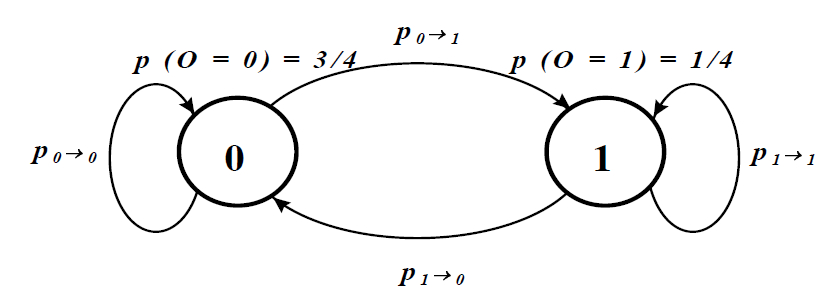
\includegraphics[width=10cm]{img/logicFSM.png}
\caption{Diagramma delle transizioni della porta NOR}\label{fig:logicFSM}
\end{figure}
Per l'output O la probabilità di transizione $p_{0\rightarrow1}$ è data dalla probabilità che lo stato corrente sia 0 e che il prossimo stato sia 1:
$$p_{0\rightarrow 1}= p(O = 0)p(O = 1)= \frac{3}{4}\times\frac{1}{4} = \frac{3}{16}$$
Così valido per gli altri stati:
$$p_{1\rightarrow 0}= p(O = 1)p(O = 0)= \frac{1}{4}\times\frac{3}{4} = \frac{3}{16}$$
$$p_{0\rightarrow 0}= p(O = 0)p(O = 0)= \frac{3}{4}\times\frac{3}{4} = \frac{9}{16}$$
$$p_{1\rightarrow 1}= p(O = 1)p(O = 1)= \frac{1}{4}\times\frac{1}{4} = \frac{1}{16}$$
Arriviamo al fattore di switching che è uguale a:
$$\alpha = p_{0\rightarrow 1} + p_{1\rightarrow 0} = \frac{3}{8}$$
\paragraph{Tecnologie}
La scelta nelle tecnologie CMOS può ricadere o in quella statica o in quella dinamica.
Nel caso di \emph{static CMOS} abbiamo che $C_L$è caricata a $V_{dd}$ ogni volta che è richiesta una transizione $0 \rightarrow 1$ all'uscita del transistor ed è scaricato a 0 ogni qualvolta vi è una transizione $1 \rightarrow 0$.\\
Nel caso di \emph{dynamic CMOS} $C_L$ è precaricato a $V_dd$ ad ogni ciclo di clock e scaricato a zero ogni qualvolta avviene una transizione $1 \rightarrow 0$. Come conseguenza di questo comportamento abbiamo che:
$$\alpha(dynamic \ CMOS) \geq \alpha(static \ CMOS)$$
e la capacità di solito è uguale a 
$$C_L(dynamic \ CMOS) \leq C_L(static \ CMOS)$$
Nel caso di static CMOS la probabilità di transizione dipende sia dalla probabilità di input sia dallo stato precedente; nel caso di dynamic CMOS invece la probabilità di switch dipende solo dalla probabilità degli ingressi.
Nel caso di static CMOS se gli input non cambiano dal ciclo di clock precedente allora le uscite non cambiano, nel caso dinamico invece gli output possono cambiare anche se gli input non cambiano.
\paragraph{Probabilità degli input}
Prendiamo il caso di una porta NOR a due ingressi implementata tramite tecnologia CMOS statica e assumiamo che gli input siano equiprobabili.
La probabilità che l'output sia uguale a 1 è data da:
$$p(O = 1) = (1-p(A = 1))(1-p(B = 1))$$
La probabilità che l'output sia 0 è data da:
$$p(O = 0) = 1 - p(O = 1)$$
La probabilità di una transizione da $0 \rightarrow 1$ è:
$$p_{0 \rightarrow 1} = p (O = 0)p(O = 1)=
(1-(1-p(A = 1))(1-p(B = 1)))(1-p(A = 1))(1 - p(B = 1))$$
\begin{figure}[hbt]
\centering
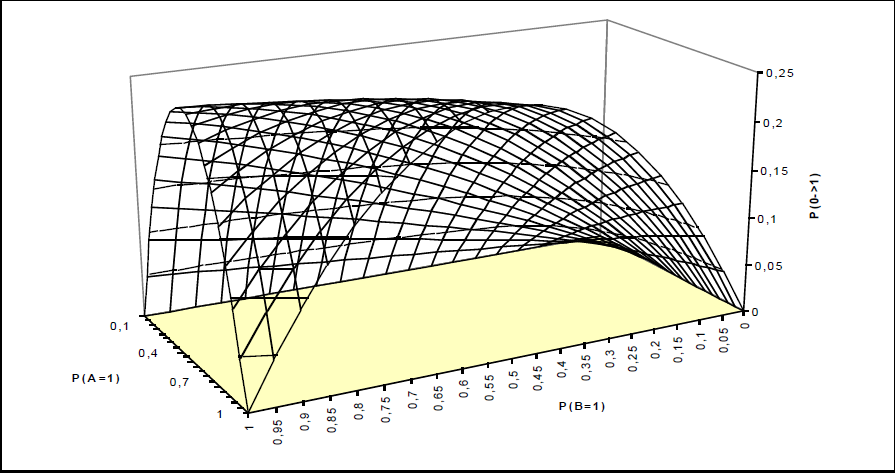
\includegraphics[scale=0.7]{img/p01.png}
\caption{Probabilità di transizione $0 \rightarrow 1$}
\end{figure}
\paragraph{Topologia del circuito} La topologia del circuito ha un forte impatto sulle attività di switching del circuito. Prendiamo ad esempio l'esempio di due implementazioni di un AND a 4 input. 
$$(1-(1-p(A = 1))(1-p(B = 1)))(1-p(A = 1))(1 - p(B = 1))$$
\begin{figure}[hbt]
\centering
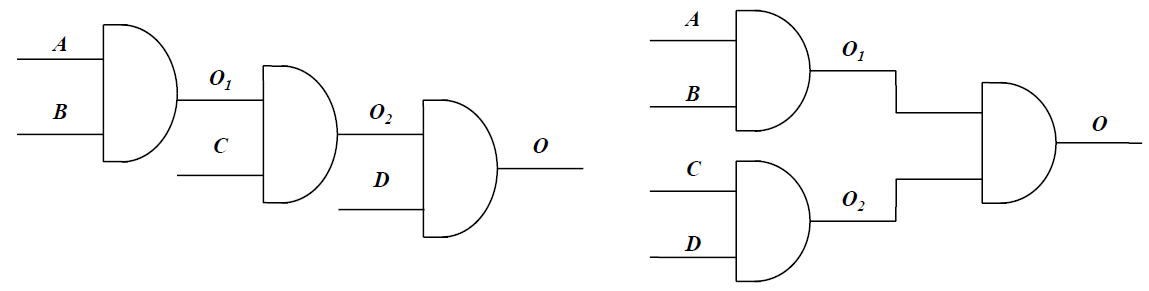
\includegraphics[scale=0.4]{img/and4input.png}
\caption{Due implementazioni di AND}
\end{figure}
Assumiamo che A,B,C,D sono indipendenti ed equiprobabili:
$$p(A = 1) = p(B = 1) = p(C = 1) = p(D = 1) = \frac{1}{2}$$
La probabilità che l'output di un AND con due ingressi sia uguale a 1 è data da:
$$p(O = 1) = p(A = 1)p(B = 1) = \frac{1}{4}$$
La probabilità che l'uscita della stessa porta sia uguale a 0 è uguale a:
$$p(O = 0) = 1-p(O = 1) = \frac{3}{4}$$
La probabilità di transizione $0 \rightarrow 1$ è data da:
$$p_{0\rightarrow 1}= p(O=0)p(O=1)§=\frac{3}{4}\frac{1}{4}=\frac{3}{16}$$
E il fattore di scambio è:
$$\alpha = p_{0\rightarrow 1} + p_{1\rightarrow 0} = \frac{3}{8}$$
Come vediamo dalla tabella in figura \ref{fig:2ANDimp}
\begin{figure}[hbt]
\centering
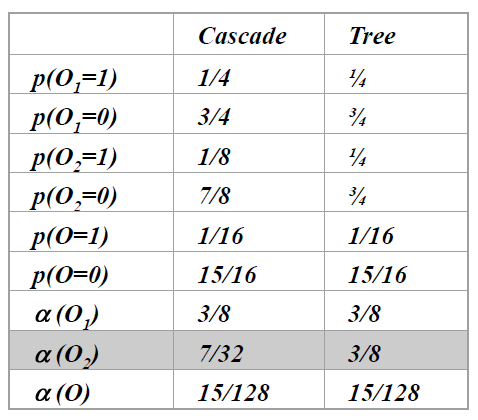
\includegraphics[scale=0.5]{img/2ANDimp.png}
\caption{Valori di comparazione per le due implementazioni di AND}\label{fig:2ANDimp}
\end{figure}
abbiamo che a parità di input la soluzione in cascata ha un fattore di switch minore.
Questo però analizzando solo i componenti statici e trascurando gli effetti di glitch che si hanno con l'analisi temporale.
\subsection{Voltage Scaling}
La velocità del circuito decresce tanto più $V_{dd}$ si avvicina a $V_{Th}$; usando una approssimazione del primo ordine possiamo modellizzare il ritardo $T_d$ del gate come:
$$T_d = \frac{C_{out}V_{dd}}{I}=\frac{C_{out}V_{dd}}{\eta(W/L)(V_{dd}-V_t)^2}$$
dove il fattore $\eta$ dipende dalla tecnologia e $W$ ed $L$ sono rispettivamente larghezza e lunghezza del canale CMOS.
L'obiettivo dei progettisti è quello di operare alla più bassa velocità possibile che permette la maggiore $V_{dd}$
Per ridurre la potenza preservando la velocità del circuito e il throughput computazionale dobbiamo ridurre l'incremento di ritardo dovuto al ridimensionamento del $V_{dd}$; esistono due approcci, il primo è quello di scalare in maniera proporzionale anche la tensione di soglia (Figura \ref{fig:thvdd}), oppure agendo sull'architettura implementando la parallelizzazione e la pipelining.
\begin{figure}[hbt]
\centering
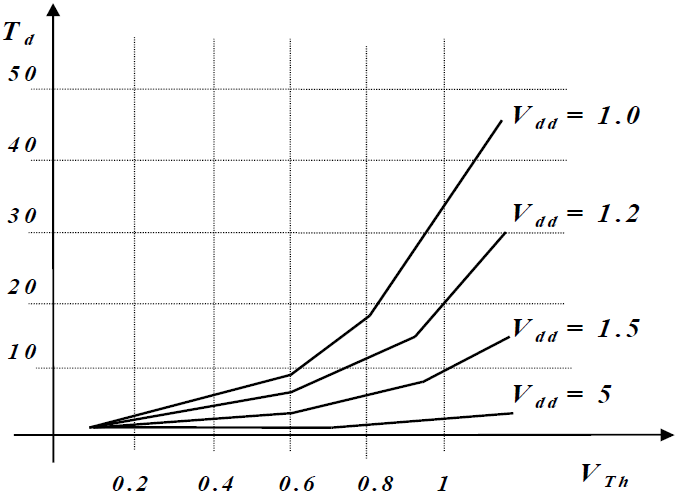
\includegraphics[scale=0.5]{img/thvdd.png}
\caption{Grafico dei ritardi in funzione di $V_{dd}$ e della tensione di soglia}\label{fig:thvdd}
\end{figure}
La riduzione della tensione di soglia permette di ridurre la potenza di switching senza perdere in velocità. I limiti sono dovuti al margine di rumore e all'incremento della corrente di sotto-strato $I_{DS}$; bisogna perciò trovare il giusto valore di bilanciamento tra la $P_{SW}$ che diminuisce al diminuire di $V_{Th}$ e $P_{Leakage}$ che invece aumenta al diminuire di $V_{Th}$
Nel caso invece di ottimizzazione dell'architettura si migliora il circuito in modo da renderlo più veloce, si riduce in seguito la $V_{dd}$ fino a ripristinare la velocità originale e si ha come effetto secondario la riduzione del consumo di energia. Come conseguenza però si ha un aumento della circuiteria che potrebbe aumentarne il consumo e parallelismo e pipelining hanno spesso un costo non indifferente.
\subsection{Tecniche di progetto a livello logico}
Analizziamo ora alcune tecniche di minimizzazione della potenza dissipata che si applicano alla progettazione a livello logico del circuito.
\subsubsection{Codifica degli stati}
Nel caso di sistemi orientati al controllo la specifica iniziale di una Macchina a Stati Finiti (FSM) è descritta tramite il Grafo di Transizione degli Stati (STG).
Il problema della codifica degli stati è quello di trovare un assegnamento di codici binari per gli stati in modo da minimizzare una determinata funzione di costo come ad esempio la potenza dissipata. Il problema è che l'assegnamento degli stati è un problema NP-completo.
Definiamo ora in modo più completo il problema della definizione degli stati; dati un STG assegnare dei codici binari agli stati in modo da minimizzare una data funzione di costo. In generale la funzione di costo C deve tener conto della distanza di \emph{Hamming} $H(s_i,s_j)$ tra i codici binari corrispondenti agli stati $s_i$ ed $s_j$ tra i quali può avvenire una transizione di stato. Una possibile funzione di costo può essere:
$$C=\sum H(s_i,s_j)$$
Una funzione di costo più accurata dovrebbe considerare altri fattori come la probabilità di transizione di stato. Come nel caso di un STG pesato i cui pesi rappresentano la probabilità di transizioni da uno stato $s_i$ ad uno $s_j$. L'idea è quello di assegnare codici \emph{vicini} a stati connessi da archi con i pesi più alti; la nuova funzione di costo diventa:
$$C = \sum W_{ij} H(s_i,s_j)$$
dove $W_{ij}$ è il peso assegnato all'arco che connette gli stati $s_i$ e $s_j$
\subsubsection{Tecniche di retiming}
La posizioni dei registri nel circuito sequenziale può impattare fortemente sull'area del circuito e di conseguenza anche sulle prestazioni e sulla potenza dissipata dal circuito. L'osservazione di base è che in un circuito sequenziale sincrono con un segnale di clock primario le uscite dei registri possono avere al più una transizione per ogni ciclo di clock. Questo riduce il numero di glitch o transizione spurie.
Le tecniche di \emph{Retiming} si basano sulla selezione di un insieme di porte logiche del circuito nei quali porre dei registri che minimizzano l'attività di transizione globale del circuito.\\
L'algoritmo è molto semplice basta selezionare un insieme di porte logiche caratterizzate da un elevato numero di glitch sulle uscite e un'alta probabilità che tali glitch si propaghino ai nodi successivi; all'uscita di queste porte si aggiunge un registro, nel caso dei registri siano già presenti nel circuito si spostano tali registri in modo da modificare la temporizzazione del circuito diminuendo la potenza dissipata ma senza impattare sulle funzionalità del circuito.
\subsubsection{Tecniche di pre-calcolo}
Sistemi digitali complessi hanno porzioni di logica che non eseguono calcoli utili  ad ogni ciclo di clock. L'idea base è quella di spegnere tale logica con l'obiettivo di limitare il consumo di potenza (\emph{logic shutdown}).\\
Nel caso del pre-calcolo si tratta di duplicare parti della logica con l'obiettivo di pre-calcolare i valori di uscita di una logica con cicli di clock in anticipo ed usare questi valori per ridurre l'attività di commutazione globale della logica durante i cicli di clock successivi.
Questo permette di spegnere la logica originale con un ciclo di anticipo. Questa tecnica però deve essere tenuta sotto controllo affinché la logica di precalcolo non diventi eccessiva.
\subsubsection{Tecniche di Clock Gating}
Le tecniche di clock gating consistono nel fermare selettivamente il segnale di clock del ciclo successivo in parti della logica dove non vengono svolti calcoli utili alla funzionalità globale del circuito.
Il segnale di clock viene disabilitato in corrispondenza di condizioni di riposo del circuito sequenziale, queste condizioni sono determinate a priori dal progettista.